\documentclass[journal,12pt,twocolumn]{IEEEtran}
%
\usepackage{setspace}
\usepackage{gensymb}
\usepackage{xcolor}
\usepackage{caption}
%\usepackage{subcaption}
%\doublespacing
\singlespacing
\usepackage{polynom}
%\usepackage{graphicx}
%\usepackage{amssymb}
%\usepackage{relsize}
\usepackage[cmex10]{amsmath}
\usepackage{mathtools}
%\usepackage{amsthm}
%\interdisplaylinepenalty=2500
%\savesymbol{iint}
%\usepackage{txfonts}
%\restoresymbol{TXF}{iint}
%\usepackage{wasysym}
\usepackage{hyperref}
\usepackage{amsthm}
\usepackage{mathrsfs}
\usepackage{txfonts}
\usepackage{stfloats}
\usepackage{cite}
\usepackage{cases}
\usepackage{subfig}
%\usepackage{xtab}
\usepackage{longtable}
\usepackage{multirow}
%\usepackage{algorithm}
%\usepackage{algpseudocode}
%\usepackage{enumerate}
\usepackage{enumitem}
\usepackage{mathtools}
%\usepackage{iithtlc}
%\usepackage[framemethod=tikz]{mdframed}
\usepackage{listings}


%\usepackage{stmaryrd}


%\usepackage{wasysym}
%\newcounter{MYtempeqncnt}
\DeclareMathOperator*{\Res}{Res}
%\renewcommand{\baselinestretch}{2}
\renewcommand\thesection{\arabic{section}}
\renewcommand\thesubsection{\thesection.\arabic{subsection}}
\renewcommand\thesubsubsection{\thesubsection.\arabic{subsubsection}}

\renewcommand\thesectiondis{\arabic{section}}
\renewcommand\thesubsectiondis{\thesectiondis.\arabic{subsection}}
\renewcommand\thesubsubsectiondis{\thesubsectiondis.\arabic{subsubsection}}

%\renewcommand{\labelenumi}{\textbf{\theenumi}}
%\renewcommand{\theenumi}{P.\arabic{enumi}}

% correct bad hyphenation here
\hyphenation{op-tical net-works semi-conduc-tor}

\lstset{
language=Python,
frame=single, 
breaklines=true,
columns=fullflexible
}


\begin{document}


\theoremstyle{definition}
\newtheorem{theorem}{Theorem}[section]
\newtheorem{problem}{Problem}
\newtheorem{proposition}{Proposition}[section]
\newtheorem{lemma}{Lemma}[section]
\newtheorem{corollary}[theorem]{Corollary}
\newtheorem{example}{Example}[section]
\newtheorem{definition}{Definition}[section]
%\newtheorem{algorithm}{Algorithm}[section]
%\newtheorem{cor}{Corollary}
\newcommand{\BEQA}{\begin{eqnarray}}
\newcommand{\EEQA}{\end{eqnarray}}
\newcommand{\define}{\stackrel{\triangle}{=}}

\bibliographystyle{IEEEtran}
%\bibliographystyle{ieeetr}

\providecommand{\nCr}[2]{\,^{#1}C_{#2}} % nCr
\providecommand{\nPr}[2]{\,^{#1}P_{#2}} % nPr
\providecommand{\mbf}{\mathbf}
\providecommand{\pr}[1]{\ensuremath{\Pr\left(#1\right)}}
\providecommand{\qfunc}[1]{\ensuremath{Q\left(#1\right)}}
\providecommand{\sbrak}[1]{\ensuremath{{}\left[#1\right]}}
\providecommand{\lsbrak}[1]{\ensuremath{{}\left[#1\right.}}
\providecommand{\rsbrak}[1]{\ensuremath{{}\left.#1\right]}}
\providecommand{\brak}[1]{\ensuremath{\left(#1\right)}}
\providecommand{\lbrak}[1]{\ensuremath{\left(#1\right.}}
\providecommand{\rbrak}[1]{\ensuremath{\left.#1\right)}}
\providecommand{\cbrak}[1]{\ensuremath{\left\{#1\right\}}}
\providecommand{\lcbrak}[1]{\ensuremath{\left\{#1\right.}}
\providecommand{\rcbrak}[1]{\ensuremath{\left.#1\right\}}}
\theoremstyle{remark}
\newcommand\Mydiv[2]{%
$\strut#1$\kern.25em\smash{\raise.3ex\hbox{$\big)$}}$\mkern-8mu
        \overline{\enspace\strut#2}$}
\newtheorem{rem}{Remark}
\newcommand{\sgn}{\mathop{\mathrm{sgn}}}
\providecommand{\abs}[1]{\left\vert#1\right\vert}
\providecommand{\res}[1]{\Res\displaylimits_{#1}} 
\providecommand{\norm}[1]{\lVert#1\rVert}
\providecommand{\mtx}[1]{\mathbf{#1}}
\providecommand{\mean}[1]{E\left[ #1 \right]}
\providecommand{\fourier}{\overset{\mathcal{F}}{ \rightleftharpoons}}
\providecommand{\ztrans}{\overset{\mathcal{Z}}{ \rightleftharpoons}}
\newcommand{\myvec}[1]{\ensuremath{\begin{pmatrix}#1\end{pmatrix}}}
\newcommand{\mydet}[1]{\ensuremath{\begin{vmatrix}#1\end{vmatrix}}}
\let\vec\mathbf
%\providecommand{\hilbert}{\overset{\mathcal{H}}{ \rightleftharpoons}}
\providecommand{\system}{\overset{\mathcal{H}}{ \longleftrightarrow}}
	%\newcommand{\solution}[2]{\textbf{Solution:}{#1}}
\newcommand{\solution}{\noindent \textbf{Solution: }}
\providecommand{\dec}[2]{\ensuremath{\overset{#1}{\underset{#2}{\gtrless}}}}
\numberwithin{equation}{section}
%\numberwithin{equation}{subsection}
%\numberwithin{problem}{subsection}
%\numberwithin{definition}{subsection}
\makeatletter
\@addtoreset{figure}{problem}
\makeatother

\let\StandardTheFigure\thefigure
%\renewcommand{\thefigure}{\theproblem.\arabic{figure}}
\renewcommand{\thefigure}{\theproblem}


%\numberwithin{figure}{subsection}

\def\putbox#1#2#3{\makebox[0in][l]{\makebox[#1][l]{}\raisebox{\baselineskip}[0in][0in]{\raisebox{#2}[0in][0in]{#3}}}}
     \def\rightbox#1{\makebox[0in][r]{#1}}
     \def\centbox#1{\makebox[0in]{#1}}
     \def\topbox#1{\raisebox{-\baselineskip}[0in][0in]{#1}}
     \def\midbox#1{\raisebox{-0.5\baselineskip}[0in][0in]{#1}}

\vspace{3cm}

\title{ Pingala Assignment
%\logo{
%}
%	\logo{Octave for Math Computing }
}
%\title{
%	\logo{Matrix Analysis through Octave}{\begin{center}\includegraphics[scale=.24]{tlc}\end{center}}{}{HAMDSP}
%}


% paper title
% can use linebreaks \\ within to get better formatting as desired
%\title{Matrix Analysis through Octave}
%
%
% author names and IEEE memberships
% note positions of commas and nonbreaking spaces ( ~ ) LaTeX will not break
% a structure at a ~ so this keeps an author's name from being broken across
% two lines.
% use \thanks{} to gain access to the first footnote area
% a separate \thanks must be used for each paragraph as LaTeX2e's \thanks
% was not built to handle multiple paragraphs
%

\author{ Mannem Charan AI21BTECH11019}
% note the % following the last \IEEEmembership and also \thanks - 
% these prevent an unwanted space from occurring between the last author name
% and the end of the author line. i.e., if you had this:
% 
% \author{....lastname \thanks{...} \thanks{...} }
%                     ^------------^------------^----Do not want these spaces!
%
% a space would be appended to the last name and could cause every name on that
% line to be shifted left slightly. This is one of those "LaTeX things". For
% instance, "\textbf{A} \textbf{B}" will typeset as "A B" not "AB". To get
% "AB" then you have to do: "\textbf{A}\textbf{B}"
% \thanks is no different in this regard, so shield the last } of each \thanks
% that ends a line with a % and do not let a space in before the next \thanks.
% Spaces after \IEEEmembership other than the last one are OK (and needed) as
% you are supposed to have spaces between the names. For what it is worth,
% this is a minor point as most people would not even notice if the said evil
% space somehow managed to creep in.



% The paper headers
%\markboth{Journal of \LaTeX\ Class Files,~Vol.~6, No.~1, January~2007}%
%{Shell \MakeLowercase{\textit{et al.}}: Bare Demo of IEEEtran.cls for Journals}
% The only time the second header will appear is for the odd numbered pages
% after the title page when using the twoside option.
% 
% *** Note that you probably will NOT want to include the author's ***
% *** name in the headers of peer review papers.                   ***
% You can use \ifCLASSOPTIONpeerreview for conditional compilation here if
% you desire.




% If you want to put a publisher's ID mark on the page you can do it like
% this:
%\IEEEpubid{0000--0000/00\$00.00~\copyright~2007 IEEE}
% Remember, if you use this you must call \IEEEpubidadjcol in the second
% column for its text to clear the IEEEpubid mark.



% make the title area
\maketitle

%\newpage

\tableofcontents

%\renewcommand{\thefigure}{\thesection.\theenumi}
%\renewcommand{\thetable}{\thesection.\theenumi}

\renewcommand{\thefigure}{\theenumi}
\renewcommand{\thetable}{\theenumi}

%\renewcommand{\theequation}{\thesection}


\bigskip

\begin{abstract}
This manual provides a simple introduction to Transforms
\end{abstract}
\section{JEE 2019}
Let 
\begin{align}
	a_n &= \frac{\alpha^{n}-\beta^{n}}{\alpha - \beta}, \quad n \ge 1
	\\
	b_n &= a_{n-1} + a_{n+1}, \quad n \ge 2, \quad b_1 =1
	\label{eq:10-orig-diff}
\end{align}
Verify the following using a python code.
\begin{enumerate}[label=\thesection.\arabic*
,ref=\thesection.\theenumi]
\item 
\begin{align}
	\sum_{k=1}^{n}a_k = a_{n+2}-1, \quad n \ge 1
\end{align}
\solution Download the following python code from the below link,
  \begin{lstlisting}
wget https://github.com/Charanyash/EE3900-Digital_Signal_Processing/tree/master/pingala/Codes/1.py
  \end{lstlisting}
Then run the following command,
  \begin{lstlisting}
python3 1.py
  \end{lstlisting}
  \begin{figure}[!ht]
 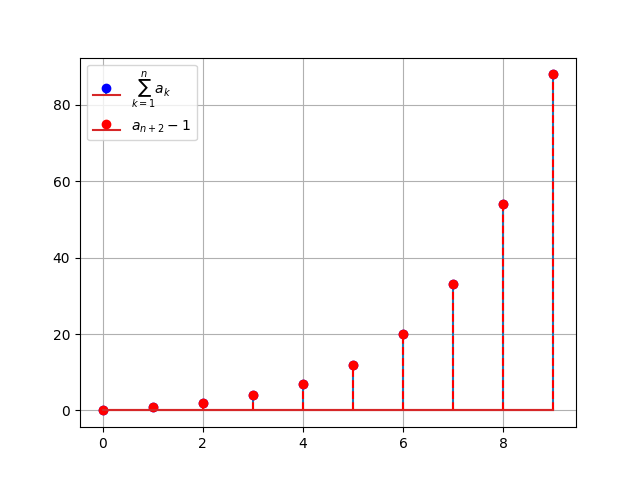
\includegraphics[width = \columnwidth]{Figs/1.1.png}
 \centering
 \caption{}
 \label{fig:1}
\end{figure}
 \item 
\begin{align}
	\sum_{k=1}^{\infty}\frac{a_k}{10^k} =\frac{10}{89}
\end{align}
 \solution
 \begin{figure}[!ht]
 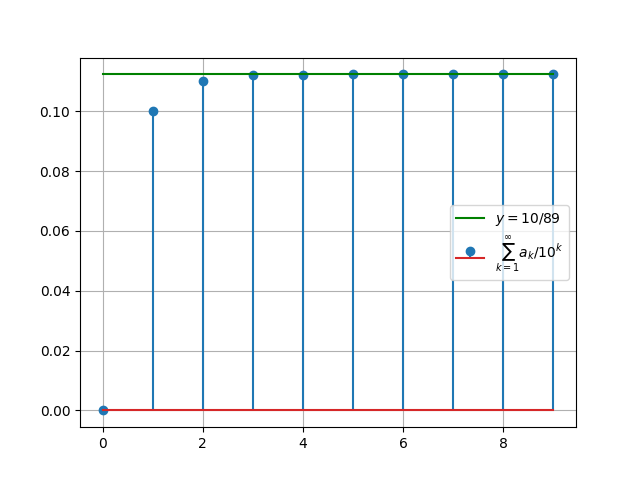
\includegraphics[width = \columnwidth]{Figs/1.2.png}
 \centering
 \caption{}
 \label{fig:2}
\end{figure}
 \item 
\begin{align}
	b_n =\alpha^n + \beta^n, \quad n \ge 1
\end{align}
 \solution
 \begin{figure}[!ht]
 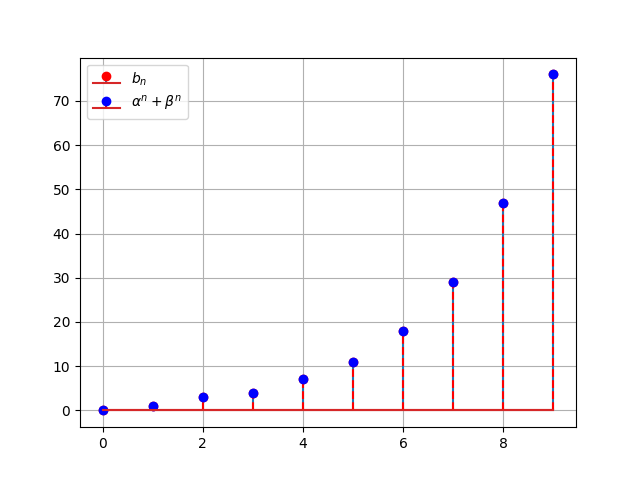
\includegraphics[width = \columnwidth]{Figs/1.3.png}
 \centering
 \caption{}
 \label{fig:3}
\end{figure}
 \item 
\begin{align}
	\sum_{k=1}^{\infty}\frac{b_k}{10^k} =\frac{8}{89}
\end{align}
\solution As you can see in the $\ref{fig:4}$, the summation is converging to $\frac{12}{89}$ but not $\frac{8}{89}$.
\begin{figure}[!ht]
 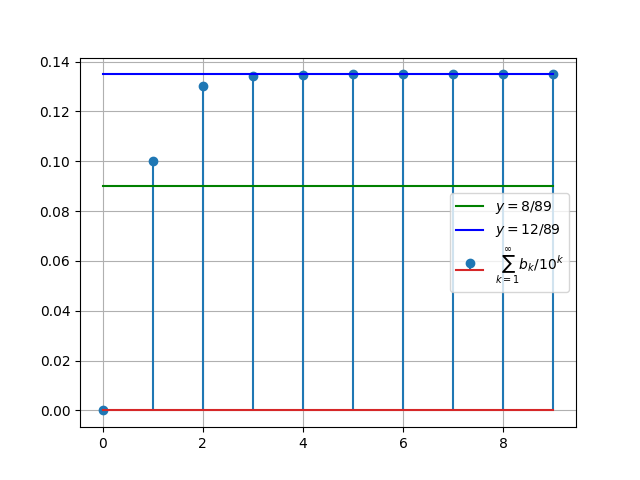
\includegraphics[width = \columnwidth]{Figs/1.4.png}
 \centering
 \caption{}
 \label{fig:4}
\end{figure}
\end{enumerate}
\section{Pingala Series}
\begin{enumerate}[label=\thesection.\arabic*,ref=\thesection.\theenumi]
\item The {\em one sided} $Z$-transform of $x(n)$ is defined as 
%\cite{proakis_dsp}
\begin{align}
	X^{+}(z) = \sum_{n = 0}^{\infty}x(n)z^{-n}, \quad z \in \mathbb{C}
\label{eq:one-Z}
\end{align}
	\item The {\em Pingala} series is generated using the difference equation 
\begin{align}
	x(n+2) = x\brak{n+1} + x\brak{n},  \quad x(0) = x(1) = 1, n \ge 0
	\label{eq:10-pingala}
\end{align}
Generate a stem plot for $x(n)$.\\
\solution Download the below python code,
  \begin{lstlisting}
wget https://github.com/Charanyash/EE3900-Digital_Signal_Processing/tree/master/pingala/Codes/2.py
  \end{lstlisting}
  Then run the following command,
  \begin{lstlisting}
python3 2.py
\end{lstlisting}
\begin{figure}[!ht]
 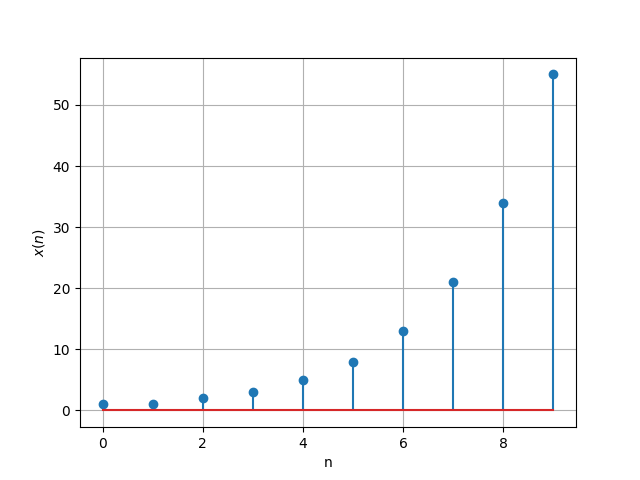
\includegraphics[width = \columnwidth]{Figs/2.2.png}
 \centering
 \caption{}
 \label{fig:5}
\end{figure}

\item 	Find $X^{+}(z)$.\\
	\solution Consider the eq :$\eqref{eq:10-pingala}$,
	  \begin{align}
		x(n+2) &= x(n+1) + x(n)
	  \end{align}
	  Now apply one-sided $Z$-transform on both sides,$(\text{using linearity})$
         \begin{align}
		 \sum_{n=0}^{\infty}x(n+2)z^{-n} = \sum_{n=0}^{\infty}x(n+1)z^{-n} + \sum_{n=0}^{\infty}x(n)z^{-n} 
         \end{align}
	 \begin{align}
		 z^2\brak{X^{+}(z) - x(1)z^{-1} - x(0)} &= z\brak{X^{+}(z) - x(0)} + X^{+}(z)
	 \end{align}
	 \begin{align}
		 X^{+}(z) &= \frac{x(1)z + x(0)\brak{z^2 - z}}{z^2 - z -1} \\
		 \implies X^{+}(z) &= \frac{1}{1-z^{-1}-z^{-2}} \label{eq:X_z} \brak{\abs{z} \neq 0}
	 \end{align}
	\item Find $x(n)$. \\
	 \solution We know that,
	  \begin{align}
            X^{+}(z) &= \frac{1}{1-z^{-1}-z^{-2}} 
          \end{align}
	  Using partial fractions,
	   \begin{align}
		   &= \frac{1}{\brak{1-\alpha z^{-1}}\brak{1-\beta z^{-1}}} \\
		   &= \frac{1}{\alpha - \beta}\brak{\frac{\alpha}{1-\alpha z^{-1}} - \frac{\beta}{1-\beta z^{-1}}}
	   \end{align}
	     where $\alpha , \beta$ are the roots of the equation,
	      \begin{align}
		      z^2 - z -1 =0
	      \end{align}
          Using the result of $Z$-transform,
	  \begin{align}
	   a^nu(n) \ztrans \frac{1}{1-az^{-1}} \quad \abs{z} > \abs{a} \\
          \end{align}
	      We can write, 
	      \begin{align}
		      x(n) &= \frac{\alpha^{n+1} - \beta^{n+1}}{\alpha -\beta}\label{eq:x_n} 
	      \end{align}
	      with ROC as,
	          \begin{align}
			  \abs{z} > \text{max}\cbrak{\alpha,\beta}
		  \end{align}
	\item Sketch 
\begin{align}
	y(n)	 = x\brak{n-1} + x\brak{n+1},  \quad n \ge 0
	\label{eq:10-orig-diff-rev}
\end{align}

\solution Download the below python code,
  \begin{lstlisting}
wget https://github.com/Charanyash/EE3900-Digital_Signal_Processing/tree/master/pingala/Codes/2.py
  \end{lstlisting}
  Then run the following command,
  \begin{lstlisting}
python3 2.py
\end{lstlisting}
\begin{figure}[!ht]
 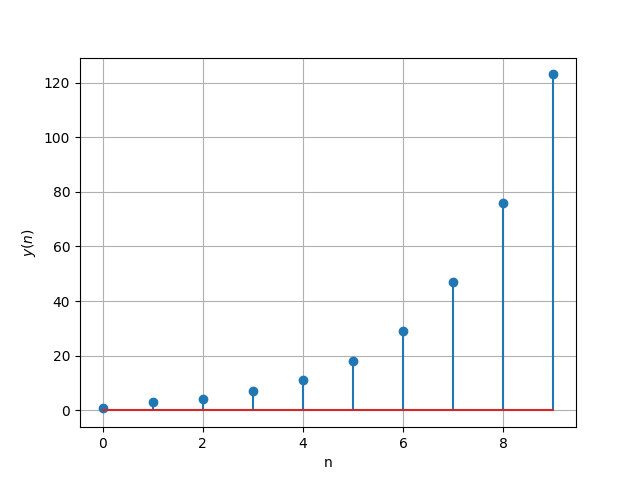
\includegraphics[width = \columnwidth]{Figs/2.5.png}
 \centering
 \caption{}
 \label{fig:6}
\end{figure}
\item Find $Y^{+}(z)$.\\
 \solution Apply the one-sided $Z$-transform on $\eqref{eq:10-orig-diff-rev}$,
  \begin{align}
       \sum_{n=0}^{\infty}y(n)z^{-n} &= \sum_{n=0}^{\infty}x(n-1)z^{-n} + \sum_{n=0}^{\infty}x(n+1)z^{-n} \\
                                     &= z^{-1}\brak{X^{+}(z) - x(-1)} + z\brak{X^{+}(z) - x(0)} 
  \end{align}
  Using $\eqref{eq:10-pingala}$ and $\eqref{eq:X_z}$,
   \begin{align}
	   Y^{+}(z) &= \frac{z^{-1}}{1-z^{-1}-z^{-2}} + \frac{1 + z^{-1}}{1 - z^{-1}-z^{-2}} \\
	   \implies Y^{+}{z} &= \frac{1+ 2z^{-1}}{1-z^{-1}-z^{-2}} \label{eq:Y_z}
   \end{align}
\item Find $y(n)$. \\
	\solution Consider $\eqref{eq:Y_z}$,
	 \begin{align} 
             Y^{+}{z} &= \frac{1+ 2z^{-1}}{1-z^{-1}-z^{-2}} \\
	              &= X^{+}(z) + 2z^{-1}X^{+}(z)
	 \end{align}
	Using $\eqref{eq:x_n}$ and the property of z-transform that,
	 \begin{align}
		 x(n-1) \ztrans z^{-1}X^{+}(z)
         \end{align}
      we can write the inverse z-transform of $Y^{+}(z)$ (using ROC as $\abs{z} > \text{max}\cbrak{\alpha,\beta}$) as,
        \begin{align}
		y(n) &= x(n) + 2x(n-1) \\
		     &=  \frac{\alpha^{n+1} - \beta^{n+1}}{\alpha -\beta} + 2 \frac{\alpha^{n} - \beta^{n}}{\alpha -\beta} \\
		     &= \frac{\alpha^{n+2} + \alpha^{n} - \beta^{n+2} - \beta^{n}}{\alpha - \beta} \\
		     &= \frac{\alpha^{n+2} - \beta^{n+2} -\beta\alpha^{n+1} + \beta^{n+1}\alpha}{\alpha-\beta} \brak{\because \alpha\beta = -1} \\
	 \implies y(n) &= \alpha^{n+1} + \beta^{n+1}
	\end{align}
\end{enumerate}
\section{Power of the Z transform}
\begin{enumerate}[label=\thesection.\arabic*,ref=\thesection.\theenumi]
\item Show that 
\begin{align}
	\sum_{k=1}^{n}a_k = 
	\sum_{k=0}^{n-1}x(n) = x(n)*u(n-1)
\end{align}
\item Show that 
\begin{align}
a_{n+2}-1, \quad n \ge 1
\end{align}
can be expressed as 
\begin{align}
	\sbrak{x\brak{n+1}-1}u\brak{n}
\end{align}
 \item Show that 
\begin{align}
	\sum_{k=1}^{\infty}\frac{a_k}{10^k}= 
	\frac{1}{10}\sum_{k=0}^{\infty}\frac{x\brak{k}}{10^k} =\frac{1}{10}X^{+}\brak{{10}}
\end{align}
 \item Show that 
\begin{align}
	\alpha^n + \beta^n, \quad n \ge 1
\end{align}
can be expressed as 
\begin{align}
	w(n) =\brak{\alpha^{n+1} + \beta^{n+1}}u(n)
\end{align}
		and find $W(z)$.

 \item Show that 
\begin{align}
	\sum_{k=1}^{\infty}\frac{b_k}{10^k} =
	\frac{1}{10}\sum_{k=0}^{\infty}\frac{y\brak{k}}{10^k} =\frac{1}{10}Y^{+}\brak{{10}}
\end{align}
\item Solve the JEE 2019 problem.

\end{enumerate}


\end{document}t
